\documentclass[french]{article}
\usepackage[T1]{fontenc}
\usepackage{fullpage}
\usepackage{babel}
\usepackage{hyperref}
\usepackage{graphicx}
\usepackage[justification=centering]{caption}
\usepackage{amsmath}
\usepackage{amssymb}
\usepackage{listings}
\usepackage{xcolor}
\usepackage{parskip}

\lstset{
    inputencoding = utf8,  % Input encoding
    extendedchars = true,  % Extended ASCII
    literate      =        % Support additional characters
      {á}{{\'a}}1  {é}{{\'e}}1  {í}{{\'i}}1 {ó}{{\'o}}1  {ú}{{\'u}}1
      {Á}{{\'A}}1  {É}{{\'E}}1  {Í}{{\'I}}1 {Ó}{{\'O}}1  {Ú}{{\'U}}1
      {à}{{\`a}}1  {è}{{\`e}}1  {ì}{{\`i}}1 {ò}{{\`o}}1  {ù}{{\`u}}1
      {À}{{\`A}}1  {È}{{\`E}}1  {Ì}{{\`I}}1 {Ò}{{\`O}}1  {Ù}{{\`U}}1
      {ä}{{\"a}}1  {ë}{{\"e}}1  {ï}{{\"i}}1 {ö}{{\"o}}1  {ü}{{\"u}}1
      {Ä}{{\"A}}1  {Ë}{{\"E}}1  {Ï}{{\"I}}1 {Ö}{{\"O}}1  {Ü}{{\"U}}1
      {â}{{\^a}}1  {ê}{{\^e}}1  {î}{{\^i}}1 {ô}{{\^o}}1  {û}{{\^u}}1
      {Â}{{\^A}}1  {Ê}{{\^E}}1  {Î}{{\^I}}1 {Ô}{{\^O}}1  {Û}{{\^U}}1
      {œ}{{\oe}}1  {Œ}{{\OE}}1  {æ}{{\ae}}1 {Æ}{{\AE}}1  {ß}{{\ss}}1
      {ẞ}{{\SS}}1  {ç}{{\c{c}}}1 {Ç}{{\c{C}}}1 {ø}{{\o}}1  {Ø}{{\O}}1
      {å}{{\aa}}1  {Å}{{\AA}}1  {ã}{{\~a}}1  {õ}{{\~o}}1 {Ã}{{\~A}}1
      {Õ}{{\~O}}1  {ñ}{{\~n}}1  {Ñ}{{\~N}}1  {¿}{{?`}}1  {¡}{{!`}}1
      {°}{{\textdegree}}1 {º}{{\textordmasculine}}1 {ª}{{\textordfeminine}}1
      {£}{{\pounds}}1  {©}{{\copyright}}1  {®}{{\textregistered}}1
      {«}{{\guillemotleft}}1  {»}{{\guillemotright}}1  {Ð}{{\DH}}1  {ð}{{\dh}}1
      {Ý}{{\'Y}}1    {ý}{{\'y}}1    {Þ}{{\TH}}1    {þ}{{\th}}1    {Ă}{{\u{A}}}1
      {ă}{{\u{a}}}1  {Ą}{{\k{A}}}1  {ą}{{\k{a}}}1  {Ć}{{\'C}}1    {ć}{{\'c}}1
      {Č}{{\v{C}}}1  {č}{{\v{c}}}1  {Ď}{{\v{D}}}1  {ď}{{\v{d}}}1  {Đ}{{\DJ}}1
      {đ}{{\dj}}1    {Ė}{{\.{E}}}1  {ė}{{\.{e}}}1  {Ę}{{\k{E}}}1  {ę}{{\k{e}}}1
      {Ě}{{\v{E}}}1  {ě}{{\v{e}}}1  {Ğ}{{\u{G}}}1  {ğ}{{\u{g}}}1  {Ĩ}{{\~I}}1
      {ĩ}{{\~\i}}1   {Į}{{\k{I}}}1  {į}{{\k{i}}}1  {İ}{{\.{I}}}1  {ı}{{\i}}1
      {Ĺ}{{\'L}}1    {ĺ}{{\'l}}1    {Ľ}{{\v{L}}}1  {ľ}{{\v{l}}}1  {Ł}{{\L{}}}1
      {ł}{{\l{}}}1   {Ń}{{\'N}}1    {ń}{{\'n}}1    {Ň}{{\v{N}}}1  {ň}{{\v{n}}}1
      {Ő}{{\H{O}}}1  {ő}{{\H{o}}}1  {Ŕ}{{\'{R}}}1  {ŕ}{{\'{r}}}1  {Ř}{{\v{R}}}1
      {ř}{{\v{r}}}1  {Ś}{{\'S}}1    {ś}{{\'s}}1    {Ş}{{\c{S}}}1  {ş}{{\c{s}}}1
      {Š}{{\v{S}}}1  {š}{{\v{s}}}1  {Ť}{{\v{T}}}1  {ť}{{\v{t}}}1  {Ũ}{{\~U}}1
      {ũ}{{\~u}}1    {Ū}{{\={U}}}1  {ū}{{\={u}}}1  {Ů}{{\r{U}}}1  {ů}{{\r{u}}}1
      {Ű}{{\H{U}}}1  {ű}{{\H{u}}}1  {Ų}{{\k{U}}}1  {ų}{{\k{u}}}1  {Ź}{{\'Z}}1
      {ź}{{\'z}}1    {Ż}{{\.Z}}1    {ż}{{\.z}}1    {Ž}{{\v{Z}}}1
      % ¿ and ¡ are not correctly displayed if inconsolata font is used
      % together with the lstlisting environment. Consider typing code in
      % external files and using \lstinputlisting to display them instead.      
  }



\definecolor{codegreen}{rgb}{0,0.6,0}
\definecolor{codegray}{rgb}{0.5,0.5,0.5}
\definecolor{codepurple}{rgb}{0.58,0,0.82}
\definecolor{backcolour}{rgb}{0.95,0.95,0.92}

\lstdefinestyle{mystyle}{
    backgroundcolor=\color{backcolour},   
    commentstyle=\color{codegreen},
    keywordstyle=\color{magenta},
    numberstyle=\tiny\color{codegray},
    stringstyle=\color{codepurple},
    basicstyle=\ttfamily\footnotesize,
    breakatwhitespace=false,         
    breaklines=true,                 
    captionpos=b,                    
    keepspaces=true,                 
    numbers=left,                    
    numbersep=5pt,                  
    showspaces=false,                
    showstringspaces=false,
    showtabs=false,                  
    tabsize=2
}

\lstset{style=mystyle}
\setlength{\parindent}{0pt}

\hypersetup{
  colorlinks=true,
  linkcolor=black,
  urlcolor=blue
}

\graphicspath{ {./img/} }
\title{%
    \huge Prédire les changements climatiques  \\
    \bigskip
    \large E2 - Cas pratique \\ 
    Développeur en Intelligence Artificielle,
    titre professionnel enregistré au RNCP - École IA Microsoft by Simplon
    \vfill
    \includegraphics[width=14cm]{global_warming.jpg}
    \vfill}
\date{12 février 2024}
\author{par Vincent Papelard}

\begin{document}
    \renewcommand{\contentsname}{Table des Matières}
    \renewcommand{\refname}{Références}
    \maketitle
    \pagenumbering{arabic}
    \pagenumbering{gobble}
    \newpage
    \tableofcontents
    \newpage
    \pagenumbering{arabic}

    \section*{Introduction}

    Un grand organisme de prédiction météorologique nous contacte. 
    Afin de prédire au mieux l'évolution du climat à échelle mondiale et dans le but de sensibiliser la population au réchaffement climatique, ses dirigeants souhaitent remplacer leurs modèles de prédiction vieillissants par un modèle d'IA moderne en cherchant la meilleure précision possible. Plus spécifiquement, ils nous demandent un modèle capable de prédire l'évolution des températures moyennes sur Terre sur de longues périodes. Ils insistent notamment sur les points suivants :
    \begin{itemize}
        \item l'organisation disposant de serveurs ultra-performants, la puissance de calcul n'est pas un problème.
        \item afin d'éviter les erreurs de prédiction et pour que le public continue à faire confiance aux prédictions météorologiques, le modèle proposé devra être celui qui offre la meilleure précision.
        \item des instructions expliquant la mise en place et l'utilisation du modèle devront être fournies.
    \end{itemize}
    
    Le code associé à ce dossier est disponible \href{https://github.com/vinpap/predict_climate_change}{sur GitHub}.

    \addcontentsline{toc}{section}{Introduction}
    \section{Jeu de données}
    
    Afin de faire la démonstration du modèle retenu, nous utiliserons \href{https://www.kaggle.com/datasets/berkeleyearth/climate-change-earth-surface-temperature-data}{ce dataset}. Il rencense les températures mensuelles moyennes sur Terre depuis le XVIIIè siècle, à échelle mondiale et en des points du globe spécifiques. Ce jeu de données est issu de l'aggrégation d'une grande quantité de données historiques réalisée par l'ONG \href{http://berkeleyearth.org/about/}{Berkeley Earth}. Berkeley Earth est associé au Lawrence Berkeley National Laboratory, un laboratoire universitaire de Californie.

    Ce jeu de données a été choisi pour plusieurs raisons :
    \begin{itemize}
        \item il couvre une longue période, allant de 1750 pour les relevés les plus anciens jusqu'à 2015. Dans la mesure où nous nous intéressons à l'évolution des températures sur le long terme, il paraît important de disposer de données remontant suffisamment loin dans le passé.
        \item il provient d'une source fiable : Berkeley Earth est une organisation reconnue par le gouvernement américain dont la direction est majoritairement composée de chercheurs.
        \item les données fournies sont des moyennes mensuelles de température. Cette granularité nous permet de capturer des informations sur l'évolution des températures au fil des saisons, ce que ne permettraient pas des moyennes annuelles par exemple.
    \end{itemize}
    
    Nous nous intéresserons  plus spécifiquement à la \textbf{température mensuelle moyenne sur Terre} de 1860 à nos jours. Cette information est stockée dans la table GlobalTemperatures.csv (cf figure 1).
    
    \begin{figure}[h!]
        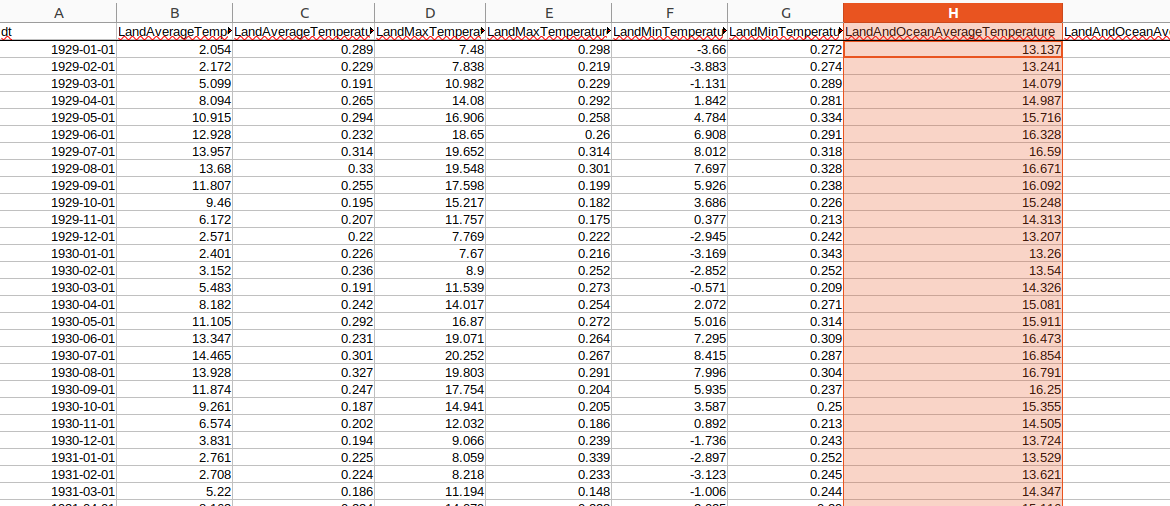
\includegraphics[width=12cm]{dataset}
        \centering
        \caption{Table GlobalTemperatures.csv}
        \centering
    \end{figure}

    Les prédictions seront réalisées avec les données de la colonne "LandAndOceanAverageTemperature" (en surbrillance sur la figure 1), qui recense la température moyenne sur Terre chaque mois, en degrés Celsius. Cette valeur est calculée en prenant en compte à la fois les températures mesurées au-dessus des continents et celles mesurées au-dessus des océans. Nous disposons ainsi d'environ 2000 valeurs, dont les premières remontent à 1850. Cette donnée nous donne donc un aperçu de la température sur Terre dans sa globalité pendant un mois donné.
    \section{Modèles de prédiction envisagés}

    Il existe de nombreux modèles d'IA qui permettent de réaliser des prédictions à partir de séries temporelles. Dans la mesure où il est impossible de tous les traiter, il a fallu faire des choix. Après recherches, les trois modèles qui seront abordés dans ce dossier sont les suivants :
    \begin{itemize}
        \item \textbf{ARIMA}
        \item \textbf{Facebook Prophet}
        \item \textbf{Réseaux LSTM (Long Short-Term Memory)}
    \end{itemize} 
    
    Ces modèles ont été spécifiquement choisis car ils sont très utilisés et qu'il existe donc beaucoup de ressources à leur sujet. Il nous sera ainsi possible de nous baser sur la littérature technique et scientifique existante pour choisir, parmi ces modèles, le plus adapté à nos besoins. Le fonctionnement de chaque modèle est exposé dans la section suivante.

    \subsection{ARIMA (Autoregressive Integrated Moving Average)}

    Plus qu'un modèle, ARIMA est une combinaison de plusieurs modèles :
    \begin{itemize}
        \item \textbf{AR - Autorégression} : ce composant calcule la valeur d'une variable à partir des $p$ dernières observations, $p$ étant un paramètre de notre modèle. Si l'on note $X_t$ la valeur de notre variable à un instant $t$, on a donc :

        \begin{equation}\forall t : X_t = \sum_{i=1}^p \alpha_i X_{t-i} + \epsilon_t \end{equation}
        avec $\epsilon$ l'erreur et $\alpha_1,...\alpha_p$ des réels.
        \item \textbf{MA - Moyenne Mobile} : la moyenne mobile (Moving Average en anglais) exprime une valeur à un instant $t$ comme une combinaison linéaire de $q$ erreurs passées :

        \begin{equation}\forall t : X_t = \epsilon_t + \sum_{i=1}^q \alpha_i \epsilon_{t-i} \end{equation}

        Pour modéliser des séries temporelles de façon plus complexe, on combine le modèle AR et le modèle MA pour créer un modèle dit "ARMA" :

        \begin{equation}\forall t : X_t = AR_t + MA_t = \sum_{i=1}^p \alpha_i X_{t-i} + \epsilon_t + \sum_{i=1}^q \beta_i \epsilon_{t-i} \end{equation}
        avec $\alpha_1,...\alpha_p$ et $\beta_1,...\beta_p$ des réels.
        \item \textbf{I - Intégration} : Le modèle ARMA a une limitation : \textbf{il ne peut modéliser que des séries de donneées stationnaires, c'est-à dire sans tendance à la baisse ou à la hausse}. Pour régler ce problème, on ajoute la composante I au modèle ARMA.
        Cette composante élimine les dépendances des données au temps en différenciant la série temporelle, c'est-à-dire en travaillant avec $X_t - X_{t-1}$ au lieu de $X_t$. Cette différenciation est réalisée $d$ fois, $d$ étant un paramètre de notre modèle ARIMA.

        \textbf{Remarque importante: }Seules certaines séries temporelles peuvent être stationnarisées grâce à la différenciation, il s'agit de celles qui ont une \textbf{racine unitaire} (PAS CLAIR, FAIRE PLUS DE RECHERCHES À CE SUJET). Il est donc important de réaliser des analyses préliminaires sur nos données pour savoir si la différenciation est adaptée à notre cas de figure avant d'appliquer le modèle ARIMA.

    \end{itemize}
    En plus des paramètres $p$, $d$ et $q$ présentés ci-dessus, le modèle ARIMA peut aussi avoir des paramètres $(P, Q, D)m$ qui décrivent la saisonnalité des données, s'il y en a une. On parle alors de modèle \textbf{SARIMA}.
    
    \subsection{Facebook Prophet}

    \href{https://facebook.github.io/prophet/}{Facebook Prophet} est un modèle de prédiction proposé par Meta. 
    Pour réaliser des prédictions, Facebook Prophet considère les données comme la combinaison additive de quatre composants\cite{meta} : 
    \begin{itemize}
        \item la tendance
        \item la saisonnalité annuelle
        \item la saisonnalité hebdomadaire
        \item une liste de jours feriés importants fournie par l'utilisateur.
    \end{itemize}
    \begin{figure}[h!]
        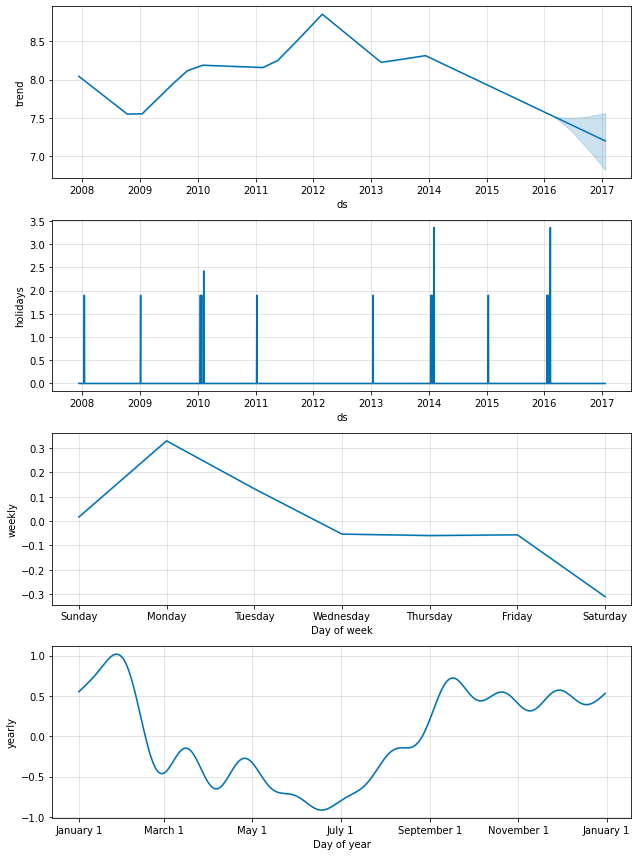
\includegraphics[width=12cm]{facebook_prophet}
        \centering
        \caption{Les différentes composantes de Facebook Prophet}
        \centering
    \end{figure}

    Chacune de ces composantes est gérée par un modèle distinct. La saisonnalité annuelle, par exemple, est modélisée à l'aide de séries de Fourier. Ces quatre modèles sont ensuite combinés additivement.
    
    Facebook Prophet se veut simple à mettre en place et permet de réaliser des prédictions très rapidement. Ce modèle était à l'origine développé pour être utilisé avec les données commerciales auxquelles sont souvent confrontés les data scientists de Meta, ce qui le rend plus adapté à certains types de données spécifiques (données financières ou commerciales par exemple). 
    
    \subsection{Réseaux LSTM (Long Short-Term Memory)}

    Le terme "LSTM" désigne un type de réseau neuronal récurrent (RNN). Les LSTM ont été créés pour pallier aux problèmes de disparition (ou d'explosion, selon les cas) du gradient souvent rencontrés lorsque l'on utilise un réseau récurrent pour traiter de longues séquences de données.
    Par rapport aux RNN classiques, les LSTM ajoutent au réseau un composant supplémentaire qui garde une mémoire de long terme, par opposition à la propagation d'informations naturellement présente dans les RNN via la réutilisation des sorties précédentes en tant que valeurs d'entrée. Les LSTM comportent des composants logiques appelés "gates" qui déterminent quels éléments doivent être stockés dans cette mémoire de long terme.

    
    \begin{figure}[h!]
        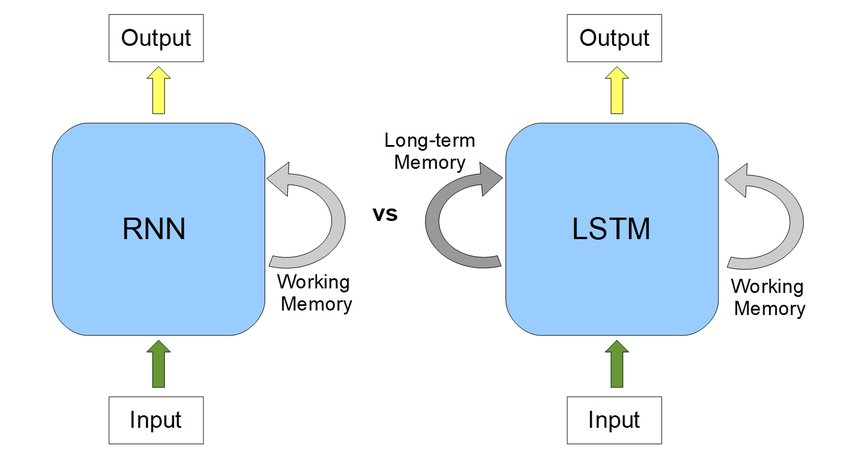
\includegraphics[width=12cm]{RNNvsLSTM}
        \centering
        \caption{Représentation d'un LSTM}
        \centering
    \end{figure}

    Loin d'être propres aux séries temporelles, les LSTM sont utilisés pour répondre à de nombreux problèmes tels que la traduction automatique, la génération de texte ou encore l'analyse de vidéos.

    \section{Comparaison des modèles}

    \subsection{Métrique utilisée}
    
    Afin de comparer les modèles considérés dans cette étude, il nous faut définir une métrique. Notre choix se portera sur la \textbf{Root-Mean-Square Error} ('racine de l'erreur quadratique moyenne' en français), souvent abrégée RMSE. Elle se définit simplement comme la racine carrée de l'erreur quadratique moyenne/mean-square error (MSE). La MSE est elle-même la moyenne du carré de l'erreur entre une valeur prédite et sa vraie valeur. Si l'on note $\check{\theta}$ la valeur prédite et $\theta$ la vraie valeur, on a :
    
    \begin{equation}RMSE(\check{\theta}) =  \sqrt{MSE(\check{\theta})} = \sqrt{E((\check{\theta} - \theta)^2)}\end{equation}

    Deux raisons expliquent ce choix :
    \begin{itemize}
        \item La RMSE est utilisée comme métrique dans la plupart des sources d'informations qui ont été utilisées dans le cadre de ce dossier
        \item La RMSE est une métrique très courante qui a l'avantage de ne pas donner une importance disproportionnée à quelques valeurs extrêmes, contrairement à la MSE.
    \end{itemize}

    \begin{figure}[h!]
        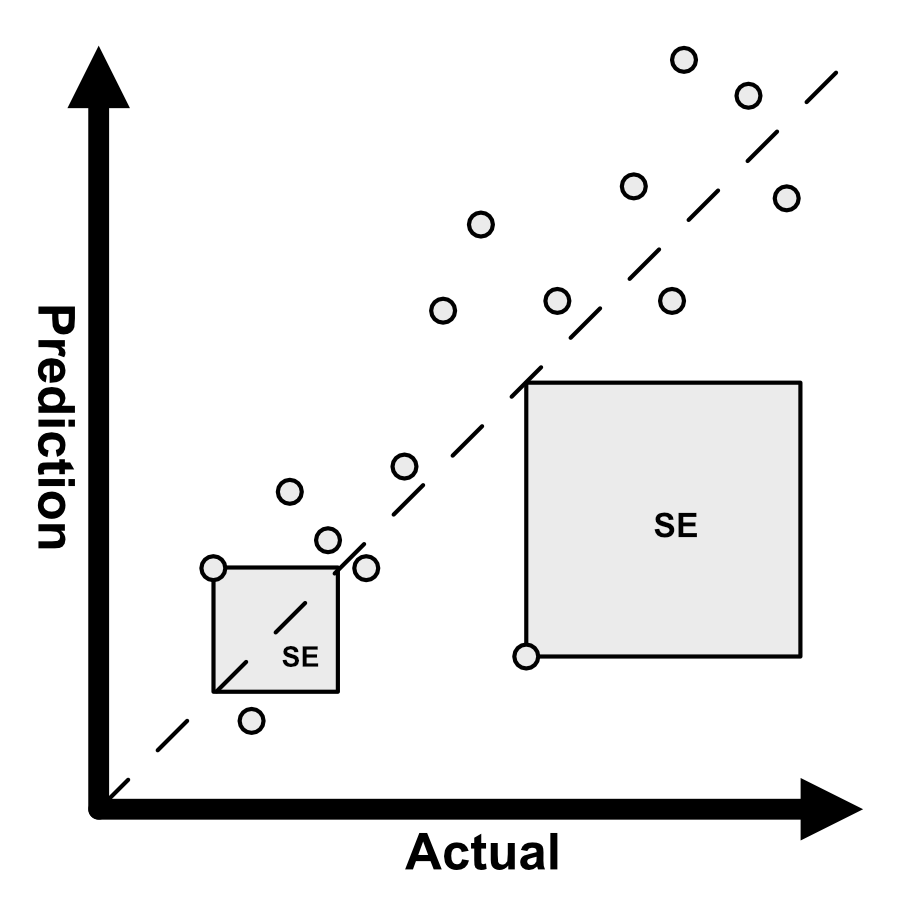
\includegraphics[width=12cm]{mse}
        \centering
        \caption{Schématisation du concept de la MSE. La MSE correspond ici à la moyenne des surfaces de tous les carrés. Pour obtenir la RMSE il suffit de calculer la racine carrée de la MSE}
        \centering
    \end{figure}

    \subsection{Présentation des sources}

    Les comparaisons ci-dessous s'appuient sur les travaux publiés dans des publications scientifiques et des sites web spécialisés dont la liste complète est disponible dans la bibliographie. Parmi ceux-là, on pourra notamment citer :
    \begin{itemize}
        \item Une étude par Ziyar Uzel et al., de la Delft University of Technology\cite{uzel}, qui compare les trois modèles pour la prévision de traffic 
        \item Une comparaison d'ARIMA, de Facebook Prophet et de modèles combinant le LSTM à des CNN, par Lorenzo Menculini et al.\cite{menculini}. Ces modèles sont appliqués à la prédiction de prix de vente de produits alimentaires
        \item Un article du fournisseur de soutions de MLOps Neptune.ai\cite{neptune} qui compare les performances de ces modèles sur des données boursières.
    \end{itemize}

    \subsection{Conclusions des sources choisies}
    Bien que toutes les sources n'arrivent pas à un consensus évident, on peut tout de même en dégager plusieurs conclusions.
    L'étude de Ziyar Uzel et al.\cite{uzel} sur les données de traffic montre que :
    \begin{itemize}
        \item ARIMA offre les meilleures performances, suivi des LSTM puis de Facebook Prophet.
        \item Pour expliquer la supériorité d'ARIMA sur les LSTM dans le contexte, l'auteur émet l'hypothèse que le dataset n'est pas assez grand pour les LSTM. Il suppose par ailleurs que le LSTM a de moins bonnes performances car son architecture ne comporte aucune information spatiale qui serait pertinente pour prédire le traffic.
    \end{itemize}
    La table 1 présente la RMSE (\textit{Root Mean-Squared Error}) obtenue avec chaque modèle.
    \begin{table}[h!]
        \begin{center}
            \begin{tabular}{ |c|c| }
                \hline
                Modèle & RMSE \\
                \hline
                ARIMA & 5.5 \\ 
                \hline
                LSTM & 7.13 \\  
                \hline
                Facebook Prophet & 8.02 \\
                \hline
            \end{tabular}
            \caption{RMSE obtenue avec chaque modèle (métrique calculée sur les données de test après finetuning) - Ziyar Uzel et al.}
            \label{table:1}
        \end{center}
    \end{table}
    
    Dans leur étude réalisée à l'Univesité de Perugia sur les prix de vente de produits alimentaires, Lorenzo Menculini et al.\cite{menculini} arrivent aux conclusions suivantes en comparant les performances des trois modèles :
    \begin{itemize}
        \item  Facebook Prophet produit des prédictions moins précises que les LSTM et ARIMA. Cependant, le modèle s'avère très simple et rapide d'utilisation, sans avoir besoin de beaucoup de nettoyage préalable sur les données.
        \item Les LSTM ont les meilleurs performances des trois modèles testés, mais aussi un temps d'entraînement largement plus long.
        \item ARIMA a une précision supérieure à Facebook Prophet et inférieure au LSTM, mais un temps d'entraînement très court comparé à ces derniers.
    \end{itemize}
    Voici les performances calculées pour chaque modèle dans le cadre de cette étude. On remarquera que les modèles ont été testés sur trois produits différents.
    \begin{table}[h!]
        \begin{center}
            \begin{tabular}{ |c| c| c| c| }
                \hline
                Produit & 1 & 2 & 3 \\
                \hline
                ARIMA & 0.0758 & 0.173 & 0.215 \\ 
                \hline
                LSTM & 0.0613 & 0.162 & 0.200 \\  
                \hline
                Facebook Prophet & 0.0812 & 0.220 & 0.350 \\
                \hline
            \end{tabular}
            \caption{RMSE obtenue avec chaque modèle (métrique calculée sur les données de test après finetuning) - Lorenzo Menculini et al.}
            \label{table:1}
        \end{center}
    \end{table}
    
    Enfin, dans son article publié sur neptune.ai\cite{neptune}, \href{https://www.linkedin.com/in/konstantin-kutzkov-%F0%9F%87%BA%F0%9F%87%A6-10a98667/?originalSubdomain=bg}{Konstantin Kutzkov} compare les trois modèles avec des données boursières. Les conclusions sont les suivantes :
    \begin{itemize}
        \item ARIMA offre les meilleures performances, suivi de Facebook Prophet puis des LSTM
        \item La sélection des hyperparamètres d'ARIMA et des LSTM a un impact considérable sur les performances du modèle.
    \end{itemize}

    La table 3 présente les résultats obtenus par chaque modèle.
    \begin{table}[h!]
        \begin{center}
            \begin{tabular}{ |c|c| }
                \hline
                Modèle & RMSE \\
                \hline
                ARIMA & 224.324 \\ 
                \hline
                LSTM & 694.612 \\  
                \hline
                Facebook Prophet & 317.081 \\
                \hline
            \end{tabular}
            \caption{RMSE obtenue avec chaque modèle (métrique calculée sur les données de test après finetuning) - Konstantin Kutzkov, Neptune.AI}
            \label{table:1}
        \end{center}
    \end{table}

    \subsection{Bilan et choix du modèle}
    À l'aide des informations ci-dessus, nous pouvons maintenant choisir en toute connaissance de cause le meilleur modèle pour notre problématique.

    Comme nous l'avons dit en début de dossier, les performances sont le critère le plus important dans notre choix, avant la facilité d'utilisation et la rapidité de mise en place. Facebook Prophet paraît donc inadapté à notre problème, au vu de ses performances inférieures à celles des autres modèles.

    En termes de performances, ARIMA et les LSTM paraissent sur un pied d'égalité. Cependant, ARIMA semble être un meilleur choix. En effet, le LSTM a besoin de beaucoup de données pour produire de bons résultats. Or, notre dataset contient une seule série de 2000 échantillons, avec une seule feature. Cela risque de ne pas être suffisant pour obtenir des prédictions fiables. Notre choix se portera donc sur un modèle ARIMA (plus précisément sur un modèle \textbf{SARIMA}, puisque nos données comportent une saisonnalité).
    
    \section{Mise en place d'ARIMA}

    Cette section couvre la mise en place d'un modèle ARIMA, de l'entraînement du modèle à sa mise à disposition sur une API. Le code relatif à cette partie du rapport est disponible dans les \hyperref[sec:code]{annexes}.

    \subsection{Chargement des données et analyses préliminaires}

    La première étape consiste à charger nos données. Pour cela, nous utiliserons \textbf{pandas} pour lire le CSV qui contient nos données et enregistrer celles qui nous intéressent dans une dataframe. 

    Comme nous l'avons fait remarquer dans la section qui traite du modèle ARIMA, la différenciation réalisée par le modèle ne permet pas de stationariser tous les types de séries temporelles. Pour nous assurer que la différenciation est bien adaptée à notre cas, nous allons réaliser une différenciation sur nos données, puis tester leur stationarité.
    La stationarité d'une série de données peut être mesurée à l'aide du \textbf{test augmenté de Dickey-Fuller}, ou test ADF. Ce test génère une p-value qui nous servira à déterminer si nos données sont stationnaires ou non. Si notre p-value est inférieure à un seuil fixé à 0.05, nos données sont stationaires. Sinon, elles ne le sont pas.
    Dans notre cas, réaliser une seule différenciation nous a permis de stationnariser nos données (voir la figure 5). Le modèle ARIMA est donc bien applicable à nos données. Par ailleurs, nous avons appris que le paramètre d de notre modèle doit prendre la valeur 1.
    \begin{figure}[h]
        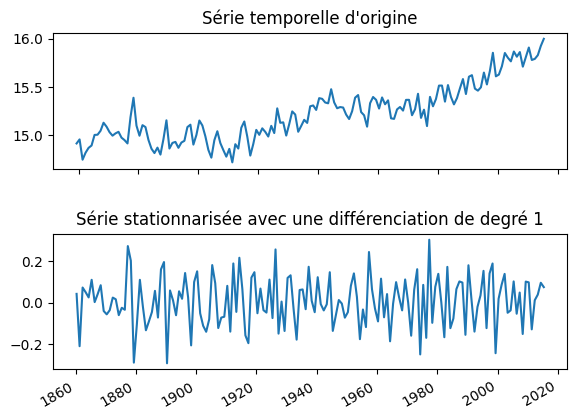
\includegraphics[width=12cm]{differenciating}
        \centering
        \caption{Visualisation de nos données, avant et après différenciation. Ici, réaliser une différenciation a permis de rendre la série temporelle stationnaire}
        \centering
    \end{figure}
    \subsection{Entraînement du modèle et sélection des hyperparamètres}

    Nous utiliserons l'implémentation de modèle SARIMA proposée par le module \href{https://pypi.org/project/pmdarima/}{pmdarima}. Ce module propose la fonction pmdarima.arima.auto\_arima, qui recherche automatiquement les meilleurs paramètres pour notre modèle.
    L'exécution de notre code nous donne la sortie suivante : \textbf{"Best model:  ARIMA(1,1,1)(2,0,1)[12] intercept"}. Les paramètres indiqués sont ceux qui offrent les meilleures performances avec notre jeu de données.

    \subsection{Prédictions}

    Nous pouvons maintenant utiliser notre modèle pour réaliser des prédictions. La figure 6 présente les prédictions obtenues par notre modèle en les confrontant avec les valeurs réelles issues de notre jeu de données de test. La lecture de ce graphique nous laisse penser que le modèle SARIMA a bien réussi à prédire les évolutions de notre jeu de données.

    \begin{figure}[h]
        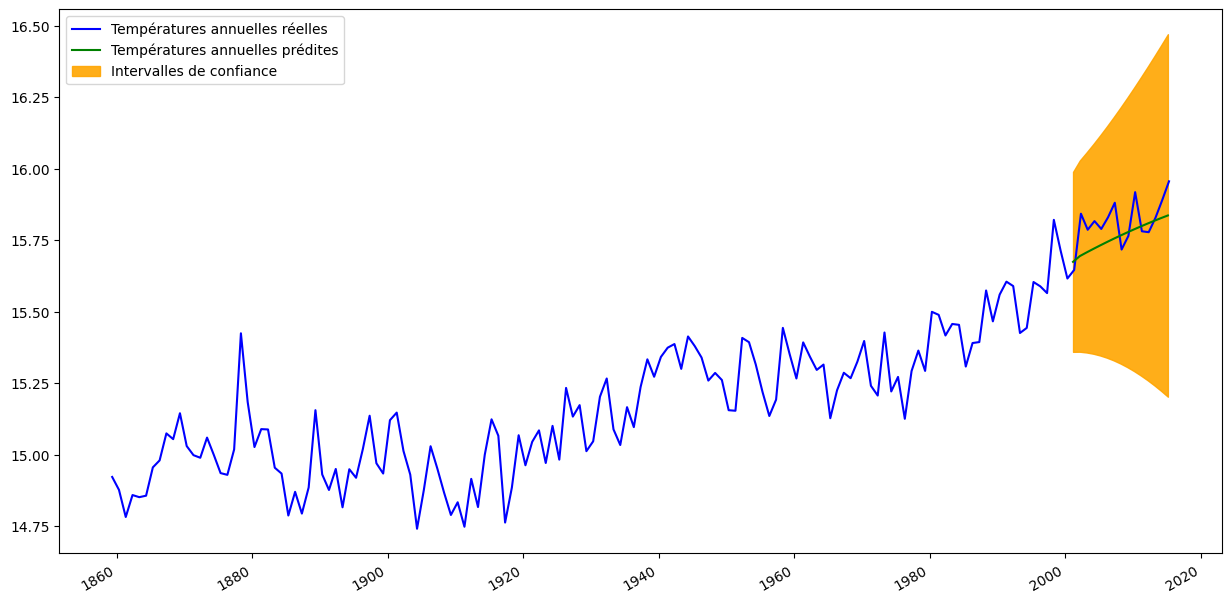
\includegraphics[width=12cm]{forecast}
        \centering
        \caption{Prédictions de notre modèle SARIMA}
        \centering
    \end{figure}

    \subsection{Monitoring du modèle}
    
    Une fois notre modèle entraîné, il est important de mettre des mécanismes en place pour s'assurer que ses prédictions restent suffisamment précises sur la durée. En effet, un problème courant lorsque l'on travaille avec des modèles de séries temporelles est le \textbf{data drift}. Le data drift désigne le phénomène qui arrive lorsque la relation entre nos valeurs prédites $Y$ et nos features $X$ change au fil du temps. Le data drift est particulièrement courant lorsque l'on travaille avec des données non stationnaires, comme dans notre cas.
    \begin{figure}[h]
        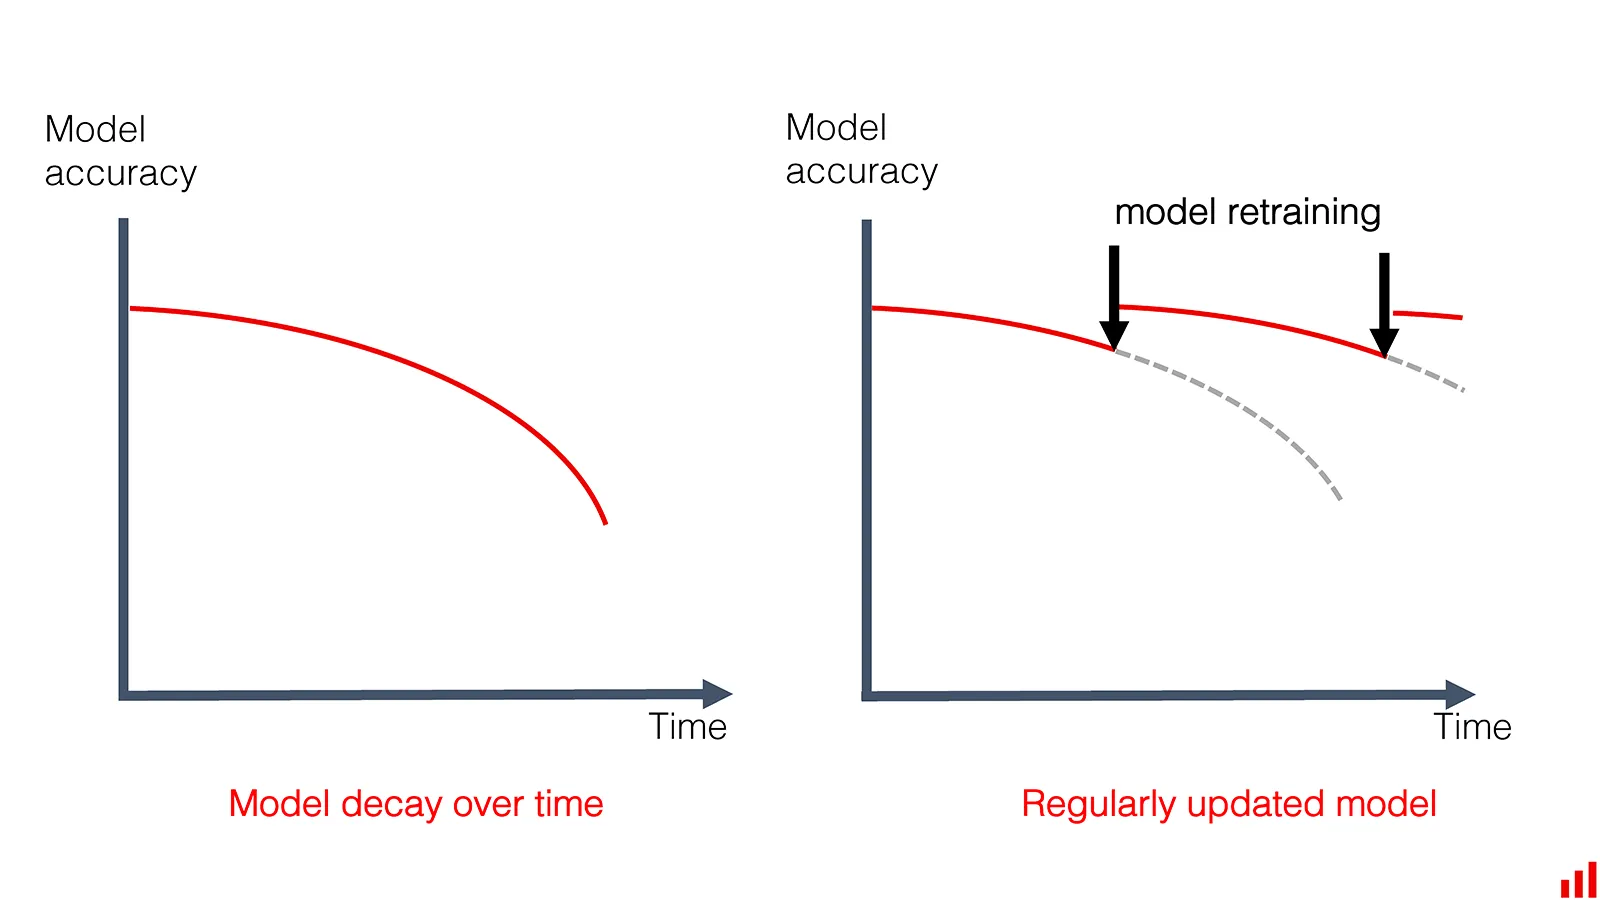
\includegraphics[width=12cm]{data_drift}
        \centering
        \caption{Illustration du phénomène de "data drift" : il faut surveiller les performances de notre modèle pour le réentraîner lorsque celles-ce se dégradent trop}
        \centering
    \end{figure}
    Une façon de se protéger du data drift est de régulièrement évaluer les prédictions de notre modèle. Si la RMSE de ces prédictions passe au-dessus d'un certain seuil, il devient alors nécessaire de réentraîner notre modèle avec des données récentes. On choisira ici d'utiliser comme seuil la RMSE de notre modèle après son premier entraînement. Un script dédié au monitoring de notre modèle sera ainsi exécuté automatiquement à intervalles réguliers. Ce script, qui aura accès aux températures mensuelles moyennes relevées récemment, réalisera des tests de notre modèle en confrontant les valeurs prédites aux relevés de température. Si la RMSE calculée est supérieure à notre seuil d'erreur défini, le script lance alors un réentraînement du modèle, en mettant à jour son jeu d'entraînement avec les derniers relevés.
    
    Pour fonctionner ce script aura besoin d'accéder aux derniers relevés de température, qui pourront être stockés dans une base de données. Le script lui-même pourra être déployé sur un service tel qu'Azure Function, qui s'occupera de l'exécuter à intervalles réguliers.


    \subsection{Déploiement}

    Il est temps de déployer le modèle sur une API afin de le mettre à disposition des météorologues. Pour cela, nous utiliserons le module Python \href{https://fastapi.tiangolo.com/}{FastAPI}, qui nous permet de réaliser rapidement des API performantes.
    Dans notre cas, nous aurons besoin de définir les endpoints suivants :
    \begin{itemize}
        \item \textbf{predict} : permet de prédire toutes les températures moyennes mensuelles comprises dans une plage de dates
        \item \textbf{train} : entraîne le modèle SARIMA
        \item \textbf{test} : prédit les températures mensuelles moyennes dans une plage de dates, puis compare ces prédictions aux températures relevées aux mêmes dates et calcule la RMSE.
    \end{itemize}

    Un point crucial est qu'il est nécessaire de \textbf{sécuriser notre API}. En l'état, celle-ci souffre d'un défaut majeur : n'importe qui peut effectuer des requêtes à notre API. Imaginons que quelqu'un sans aucun rapport avec l'organisation de météorologie que nous servons réentraîne le modèle avec ses données, ou sature les capacités de la machine qui héberge notre API en réalisant de nombreuses requêtes simultanément : ce serait un désastre !

    Pour résoudre ce problème, nous allons implémenter un contrôle d'accès à l'aide d'un \textbf{token de sécurité}. Ce token devra être envoyé avec chaque requête à notre API. Seules les requêtes qui présentent un token valide seront traitées ! On veillera par ailleurs à ne pas stocker de token en clair dans le code de notre API. Il serait envisageable de conserver nos valeurs secrètes dans les variables d'environnement de la machine qui héberge notre API, ou sur un service dédié tel qu'Azure Vault. 


    La figure 8 récapitule le fonctionnement de notre API et ses interactions avec les autres composants.

    \begin{figure}[h]
        \includegraphics[width=12cm]{schema_API_E2}
        \centering
        \caption{Fonctionnement de l'API sur laquelle est déployée notre modèle SARIMA}
        \centering
    \end{figure}

    \newpage
    \section*{Conclusion}
    Ce rapport nous a offert une présentation de trois des modèles de prédiction de séries temporelles les plus utilisés : \textbf{ARIMA}, \textbf{Facebook Prophet} et les \textbf{LSTM}. Nous avons ensuite vu pourquoi ARIMA était le modèle le plus adapté à nos besoins. Enfin, nous avons présenté comment déployer notre modèle sur une API REST pour le mettre à disposition des météorologues qui souhaitent réaliser des prédictions concernant les évolutions futures du climat.
    Sur une note plus personnelle, le travail réalisé pour ce projet m'a permis de mieux comprendre le fonctionnement des modèles de séries temporelles ainsi que les caractéristiques propres à ce type de données.

    Pour aller plus loin, n'hésitez pas à consulter les exemples de code joints aux annexes de ce dossier. L'intégralité du code source développé dans le cadre du dossier est quant à lui disponible sur \href{https://github.com/vinpap/predict_climate_change}{GitHub}.

    \addcontentsline{toc}{section}{Conclusion}

    \newpage
    \begin{thebibliography}{5}
        \bibitem[1]{uzel} ÜZEL, Ziyar. Comparative Analysis of LSTM, ARIMA, and Facebook’s Prophet for Traffic Forecasting: Advancements, Challenges, and Limitations. 2023. 
        \bibitem[2]{menculini} Menculini, L.; Marini, A.; Proietti, M.; Garinei, A.; Bozza, A.; Moretti, C.; Marconi, M. Comparing Prophet and Deep Learning to ARIMA in Forecasting Wholesale Food Prices. Forecasting 2021, 3, 644-662. https://doi.org/10.3390/forecast3030040
        \bibitem[3]{neptune} Kutzkov, Konstantin. ARIMA vs Prophet vs LSTM for Time Series Prediction. 2023. https://neptune.ai/blog/arima-vs-prophet-vs-lstm
        \bibitem[4]{medium} Tum, Phylypo. Overview of Time Series Forecasting from Statistical to Recent ML Approaches. 2020. https://medium.com/@phylypo/overview-of-time-series-forecasting-from-statistical-to-recent-ml-approaches-c51a5dd4656a
        \bibitem[5]{meta} Sean J. Taylor, Ben Letham. Prophet Forecasting at Scale. 2017. https://research.facebook.com/blog/2017/2/prophet-forecasting-at-scale/
    \end{thebibliography}

    \end{document}